\appendix
\section{Exploratory extension: opening new facility-procedure pairs}
\label{app:explore}

This appendix is exploratory. It rests on an assumed capability for new pairs, was not validated by choosing pairs on one year and evaluating them on a later one, and uses demand that omits Goi\'as residents treated in the Federal District. It supports no recommendation.

\subsection{Was capability placed where the model priced it?}
\label{sec:placement}

Because equation~\eqref{eq:cap} is a constraint rather than a bound, its dual is
available at no extra cost, and it has a direct reading: the shadow price on
$\kappa_{jp}$ is the marginal reduction in the program's objective, in index units per
month (at the 2023 optimum all demand is assigned and relaxing a cap cannot create unmet demand, so the change falls on the cost index alone), from one additional unit of permitted volume under the historical peak-cap rule at facility $j$ for
procedure $p$. In the 2023 solution 143 pairs carry a positive dual, 95 of them
non-floored, and the largest reach the ceiling of 3 index units per case,
the value of treating locally a patient who otherwise leaves their intermediate
region entirely. This is the priced object of the exploratory extension in Appendix~\ref{app:explore}, and it
requires no assumption about what opening a pair would cost.

Three properties of this dual vector should be stated before it is used. The
population is the pairs in scope, 517 of the 637 in 2023 being non-floored, which
is a larger set than the 490 used and non-floored pairs that Section~\ref{sec:formulation}
uses as the denominator for binding shares: a pair carrying no flow is still a
candidate for capability. The dual vector is degenerate. Of the 249 non-floored
pairs at their cap in 2023, only 95 carry a positive shadow price and 154 carry
zero, which is ordinary for a transport-like program with many alternative optima
and is not an error. But it means the dual vector is not unique, so any ranking
built on it is partly a property of the solver rather than of the system. We test
this directly by re-solving with the objective perturbed by uniform noise of
$10^{-4}$, twenty times. The Spearman rank correlation of the dual vector against
the unperturbed solution averages 0.73 and never falls below 0.72, and 78 per cent
of the top fifty pairs are retained on average, never fewer than 74. The ranking
is therefore informative but not sharp, and Section~\ref{sec:extension} treats a
dual-ranked list as a screen to be verified rather than as an answer.

It also supports a test. If the model has normative content, capability added
between 2023 and 2025 should have appeared disproportionately where the 2023
solution priced it highly. We rank pairs by dual times a fixed increment of five
cases per month and ask what share of subsequent capability growth landed in the
top decile, against a null in which the top decile is drawn at random with
probability proportional to facility size, so that a result cannot be produced by
large facilities simply growing more.

The literal form of this test is not identified: a pair absent from the 2023
option set has no 2023 dual, so pairs absent in 2019 cannot be scored on the
ranking they would be tested against. We run it on the two margins that are
identified. On the pair margin, across those 517 non-floored 2023 pairs, 17.1 per
cent of the 1{,}875 cases per month of subsequent growth in $\kappa_{jp}$ landed
in the top-valued decile, against a null mean of 14.1 per cent and a null 95th
percentile of 22.4 ($p = 0.26$). On the facility margin, 13.7 per cent of the 131
pairs new in 2025 appeared at the top decile of facilities by summed 2023 value,
against a null mean of 9.3 per cent and a 95th percentile of 14.5 ($p = 0.10$).

Both point the right way and neither is distinguishable from size-weighted random
placement. Whether that is informative depends on what the test could have
detected, so we report it. On the pair margin the null's 95th percentile is 22.4
per cent, and allowing for the spread of the alternative the test rejects a true
concentration of 26.5 per cent or more with 80 per cent power, against a null mean
of 14.1: it resolves a lift of about 1.9 times. On the facility margin the
corresponding figures are 14.5 and 17.0 per cent against a null mean of 9.3, again
a lift of about 1.8 times. A test that would have found capability going to the
priced pairs at roughly twice the rate chance predicts did not find it. The test's minimum detectable lift is about 1.8 to 1.9 times chance, so it does not exclude
a tilt of up to roughly that size, and pairs that are new in the later year (entrants) are excluded from it
by construction.

The test does not detect concentration of new capability at the priced pairs. Rio Verde, where local capability
more than doubled and the largest single distance from the optimum in the panel closed, is a single visible case, not a pattern the test detects.

The test finds no detectable concentration, and it could not have detected lifts below about 1.9 times chance, so we draw no conclusion about whether capability placement is aimed at the priced pairs. A ranking of the kind above
is therefore a model output, not a description of SES-GO practice or a recommendation, and Section~\ref{sec:extension} treats it accordingly.
Two cautions carry into any such use. The floor of $0.5$ generates high duals at
pairs whose cap is a construct rather than a measurement, so floored pairs must be
excluded before ranking. And where the facility total also binds, which
Section~\ref{sec:formulation} shows is the majority case, a pair's dual overstates what
relaxing that pair alone would buy.


\subsection{What a budget of new capability would buy}
\label{sec:ksweep}

Section~\ref{sec:placement} finds no detectable concentration of new capability at the priced pairs. A separate exploratory question is which pairs the program would open, and it can be posed without the pair-opening cost the data does not contain. Fix a budget of
$k$ new facility-procedure pairs, let the program choose which to open, and sweep
$k$. No price enters anywhere.

Formally, a binary $y_{jp}$ is added for each candidate pair, a pair at a facility
in $J$ for a procedure that facility does not currently perform, with
$\sum_{jp} y_{jp} \leq k$ and a cap of $y_{jp}\hat{\kappa}_{jp}$ in place of
$\kappa_{jp}$. Everything else is the program of equation~\eqref{eq:cap}
unchanged. In particular the facility total and the bed-day row still bind on
opened pairs: a facility that is already at its total cap may re-mix its caseload
but may not do more of it. That is a deliberate reading, and
Section~\ref{sec:formulation} shows it is the majority case.

Three quantities have to be assumed rather than measured, and each is stated
rather than tuned. A newly opened pair receives capability $\hat{\kappa}_{jp}$
equal to the median $\kappa_{jp}$ for that procedure among facilities in the same
bed-size tercile, swept at $0.5\times$, $1\times$ and $2\times$ as a ladder in the
manner of Table~\ref{tab:modelrobust}. A new pair has no facility-specific length
of stay and receives the procedure-level mean. And a candidate pair is linked only
to municipalities within cost 1, its facility's own municipality or immediate
region, because opening capability to serve patients two regions away is not the
policy this represents. Of 1{,}471 candidates, the 400 with the largest values in
the linear relaxation are carried into the integer program. The optimality gaps
reported below are therefore gaps on that restricted problem, and every value in
Table~\ref{tab:ksweep} is a value for that restricted problem under the three assumptions above. We
do not call the gains conservative: the capability assumed for a new pair, the candidate arcs, the stay length and the omitted
Entorno demand could each move them in either direction, and choosing pairs on one year and evaluating them on a later one
was not done.\footnote{The screen does not bind at these budgets. Across all
eleven budgets and all three $\hat{\kappa}$ levels, 81 distinct candidates are
ever selected, 55 of them at the central level, leaving 319 of the 400 screened
candidates never chosen. A screen that is never exhausted cannot be excluding a
better solution at $k \leq 50$.}

\begin{table}[t]
\centering
\caption{Reduction in optimal mean travel cost from opening $k$ new
facility-procedure pairs, 2025, as a percentage of the $k=0$ optimum of 0.642.
Columns are the assumed capability of an opened pair, as a multiple of the
tercile median. Every cell solved to a relative MIP gap below $10^{-3}$.}
\label{tab:ksweep}
\begin{tabular}{lrrr}
\toprule
& \multicolumn{3}{c}{$\hat{\kappa}$ multiplier} \\
\cmidrule(lr){2-4}
Budget $k$ & $0.5\times$ & $1\times$ & $2\times$ \\
\midrule
1  & 0.60\%  & 0.72\%  & 1.29\%  \\
2  & 1.17\%  & 1.45\%  & 2.36\%  \\
3  & 1.58\%  & 2.13\%  & 3.34\%  \\
5  & 2.35\%  & 3.40\%  & 4.93\%  \\
8  & 3.37\%  & 5.06\%  & 6.95\%  \\
12 & 4.60\%  & 6.84\%  & 9.05\%  \\
16 & 5.64\%  & 8.33\%  & 10.54\% \\
20 & 6.61\%  & 9.48\%  & 11.77\% \\
30 & 8.49\%  & 11.55\% & 13.91\% \\
40 & 9.85\%  & 13.12\% & 15.46\% \\
50 & 10.90\% & 14.26\% & 16.54\% \\
\bottomrule
\end{tabular}
\end{table}

Table~\ref{tab:ksweep} reports the frontier. The gains are large and concave.
Twenty new pairs, at the central assumption, cut the optimal mean cost index by 9.5 per cent; fifty cut it by 14.3. Put against the observed allocation, the attainable
frontier moves from 29.1 per cent below observed with the capability that exists
to 35.8 per cent at $k=20$ and 39.2 at $k=50$. In the model, twenty opened pairs widen the benchmark gap from 29.1 to 35.8 per cent of the observed index, about a quarter more than reallocation alone. These are values of an exploratory program under assumed capability for new pairs, with demand that omits Entorno residents; they are not a recommendation.

\paragraph{The choice is only partly identified.} The frontier is robust to
$\hat{\kappa}$ in shape but the identity of the chosen pairs is not, and that is a
finding rather than a nuisance. At $k=1$ the three levels choose three different
pairs, with no overlap at all; at $k=3$ the pairwise Jaccard overlaps are 0.20,
0.50 and 0.00. Which single capability is most valuable depends entirely on how
much capability one assumes it comes with, and the data does not identify that.
Agreement improves with the budget: at $k=20$ the pairwise overlaps are 0.60,
0.67 and 0.43, and twelve of the twenty pairs are chosen at all three levels.
The defensible object is therefore a set of roughly a dozen, not a ranked
shortlist of three, and any recommendation phrased as ``open this pair first''
would be reading the assumption rather than the data.

Where that core sits is itself informative. At $k=20$ under the central
assumption the openings concentrate in Luzi\^ania and Rio Verde, four each, then
Ceres and Aparecida de Goi\^ania with two, and by subgroup they are: nine in oncological surgery (0416), four in circulatory-system surgery (0406), four in musculoskeletal surgery (0408) and three in other surgeries (0415). Of the twelve pairs chosen at all three levels, six are in oncological surgery and three each in circulatory-system and musculoskeletal surgery. Under the central assumed-capability scenario and this candidate set, the exploratory model selects pairs closer to recorded demand; this is a scenario result, not evidence of which pairs should be opened. The same direction appears in Section~\ref{sec:flows}, from the flow matrix, and Section~\ref{sec:capbind}, from the binding pattern.

\paragraph{Solve times.} The three sweeps took 733, 878 and 976 seconds in total
across eleven budgets each, on a single core through HiGHS. Every cell reported
closed to a relative gap below $10^{-3}$ within a 150-second limit. An earlier
pass at a 45-second limit did not: at $\hat{\kappa} = 0.5\times$ and $k = 50$ the
solver returned a feasible point worse than doing nothing, with a relative gap of
1. That is recorded here rather than dropped, because a budget of 50 cannot be
worse than a budget of 40 and an incumbent that says otherwise is a solver
artifact, not a result.


\subsection{Validation and extension}
\label{sec:extension}

The endogenous-opening extension, deferred in earlier drafts, is no longer
outstanding.
Section~\ref{sec:ksweep} implements it under a budget rather than a price, which
is what makes it feasible: the pair-opening cost the data does not contain never
has to be supplied. What that section cannot do is compare the chosen pairs with
those that actually appeared on equal terms, because $\hat{\kappa}$ is assumed
and the choice at small budgets turns out to depend on it. A cost-based variant
would still be worth having if pair-level capital and staffing costs could be
obtained from SES-GO, which we have not attempted.

Two questions do remain, and neither is answerable with the data in hand.

First, is the 2025 plateau a constraint? State-administered facilities
plateau at approximately 151 elective cases per facility-month in the final regime (April to December 2025; mean over state-administered facility-months with elective volume) while municipal-administered facilities continue to climb, a pattern
consistent with an operating-room session constraint distinct from the bed-day
budget. The 2025 instance is solved above and has the lowest ratio of cap to demand of the three years, but the session constraint is not imposed
separately from the bed-day budget and the two cannot be distinguished on SIH
alone. Testing it requires operating-room session data the billing record does
not contain.

Second, does the objective survive replacement? The travel-penalised formulation
is the defensible choice given that SIH records no queue registration date and
therefore no waiting time. A request for aggregate queue
extracts from the state regulation system is pending. Were it to return, a
weighted-tardiness objective becomes estimable and should be reported alongside.
\section{Timing of the 2022 change and growth across facilities (descriptive)}
\label{app:timing}

These subsections describe when and where elective volume grew in 2022. They do not identify the cause of the growth.

\subsection{The 2022 change occurred in two waves}

The 2022 break date is not stable across specifications, and the instability is
informative rather than a nuisance. On the full sample PELT returns May 2022;
on the reliable subset it returns October 2022; a single-changepoint search
returns September. Running the reliable-subset series at a lower penalty
returns both May and October.

Inspection of the seasonally adjusted series shows why. The ratio is 0.334 in
January and February 2022, then 0.522, 0.493, 0.546, 0.510 and 0.505 from March
to July, then 0.665 in August. A fixed-cardinality search with two breaks over
the window June 2021 to June 2023 returns April 2022 and September 2022, with
segment means of 0.400, 0.469 and 0.633. There are two steps, not one, and
single-changepoint procedures report a date between them.

The two steps involve different sets of facilities. Classifying reliable-subset
hospitals by whether their volume grew by more than 30 per cent across the
first step (August 2021 to February 2022 against March to July 2022) or the
second (March to July 2022 against August 2022 to January 2023) gives nine
facilities that move only in the first, twelve that move only in the second,
six that move in both and twenty-two that move in neither, on the 49 facilities
clearing five elective cases per month in the August 2021 to February 2022 base
window. The correlation between the two growth ratios is $-0.04$ (Pearson),
$-0.22$ in logs and $-0.07$ by rank. Weighted by volume, second-wave movers
contribute 1{,}147 elective cases per month by late 2022 against 461 for
first-wave movers.

Two checks say this is not an artefact. Dropping the low-base rule and using all
61 facilities gives fourteen, thirteen, ten and twenty-two (59 facilities with a defined growth ratio; two are undefined), with correlations of
$+0.03$, $+0.03$ and $-0.01$. And the two ratios share the window March to July
2022, which mechanically depresses their correlation, so we split that window and
recompute with independent denominators: the first step measured to May and the
second from June. Across the full 61 and both subsets the nine resulting
correlations run from $-0.07$ to $+0.13$. The sign is not stable across these
cuts and no weight should be placed on it; what is stable is that all of them sit
near zero, and that facilities moving in both waves stay a clear minority, six of
49 and ten of 59. The movers in the two waves are uncorrelated across facilities.

The case mix, by contrast, moves the same way in both steps. Across four-digit
SIGTAP subgroups the share changes in the first and second steps correlate at
0.86: subgroup 0407 gains 2.75 and then 2.89 percentage points of share, 0415
gains 1.40 and then 1.32, while 0406 and 0416 lose share in both. In SIGTAP these are, respectively, surgery of the digestive system, annexed organs and abdominal wall (0407), whose highest-volume member is laparoscopic cholecystectomy; other surgeries (0415); surgery of the circulatory system (0406), led by bilateral varicose vein repair; and oncological surgery (0416). Geographically, the state's
largest municipality by surgical volume grows by a factor of 1.0 in the first
step and 1.4 in the second, while several interior municipalities grow by
factors between 2.5 and 4.5, at different times. This is measured at
municipality level; the \emph{regi\~ao de sa\'ude}, along which such a reform is
actually rolled out, is not carried in the SIH reduced files.

These patterns are compatible with staged policy implementation, but they do not establish that a policy caused the changes in procedure mix or the timing of facility-level growth.


\subsection{The July 2022 step came from existing facilities}
\label{sec:appb2}

The number of facilities performing elective surgery does not change at the
break. Monthly counts of distinct CNES codes with positive elective volume
range from 94 to 113 across 2022 with no discontinuity in August, against a 26
per cent increase in monthly volume between July and August. Partitioning
facilities into those active in the first half of 2022 and those not, the
July-to-August increase of 1{,}215 elective cases decomposes into 1{,}210 from
facilities already active and 5 from facilities not active in that window.
Facilities with no elective volume in the first half of 2022 remain below
2 per cent of volume through 2022.

Concentration falls. The Herfindahl-Hirschman index of elective volume across
facilities averages 479 over the pre-break window and 398 over the post-break
window; the number of facilities accounting for 90 per cent of volume moves
from the low forties in the first half of 2022 to around fifty in the second.
Volume rose without the distribution across facilities becoming more
concentrated.

The step increase was therefore obtained on the intensive margin: the same
physical facilities produced substantially more elective surgery. Whether they
did so by using existing capacity more fully or by adding staff and equipment
cannot be settled from SIH alone. Cases per surgical bed-month across the break
are reported in Section~\ref{sec:provider}, and show that the additional volume
did not exhaust the constructed bed-day budget: throughput per bed rose in both provider groups without either exhausting it. The corresponding measurement on
staffing has not been made, so activation of latent capacity and silent capacity
expansion cannot be distinguished here.

\paragraph{The longer horizon is different.} The intensive-margin finding is a
statement about the discontinuity, not about the expansion as a whole. Over the
full 2019 to 2023 interval the composition of the increase inverts. Comparing
the set of facility-procedure pairs observed in 2019 with those observed in
2023, both at the four-digit level at which the model of Section~\ref{sec:model}
routes, 284 pairs are present in 2023 and absent in 2019, carrying 21{,}845
elective cases, 27.5 per cent of 2023 volume. A further 192 pairs present in
2019 are absent in 2023, so the pair
count rises from 574 to 666 on gross churn of 476. These counts are over every
facility with elective volume. The option sets of Section~\ref{sec:model}, 563
and 637, are the same quantity restricted to facilities that also have non-zero
net surgical bed capacity, which is why their net change is 74 rather than 92. Of these, 18{,}370 cases are at facilities that report no elective
surgical volume at all in 2019, against 3{,}475 cases from procedures newly
performed at facilities already active in 2019.
A single facility accounts for the largest share: CNES 9680977 billed 3{,}185
AIH in 2019 with zero elective volume and reached 5{,}568 elective cases in
2023, a conversion of an urgent-only unit to elective provision rather than a
new entrant. Of the thirty facilities carrying the 18{,}370 cases, seventeen
appear in the 2019 SIH file with non-elective admissions, several at substantial
volume: CNES 2517949 billed 4{,}262 admissions in 2019, 2534584 2{,}416, 2442728
1{,}741 and 2769603 1{,}231. Absence from the elective data is not absence from
the system. Measured against the elective subset the extensive share is 84.1 per
cent; counting only facilities absent from SIH altogether it is 52.0 per cent.
The second is the
conservative reading and the one we rely on.

\paragraph{Endpoint-year comparisons obscure the timing of recorded activity.}
The comparison above treats a pair as a state, present in a year or absent from
it, and the monthly panel does not support that reading. Of the 284 pairs absent
in 2019, 195 are active in at least one month of 2020, 2021 or 2022, with a
median of five active months and ten cases before 2023 and 13{,}132 cases
between them. They carry 20{,}568 of the 21{,}845 cases, so of the 27.5 per cent
of 2023 volume attributed to pairs absent in 2019, 25.9 points are pairs
with activity in the intervening years, and 1.6 points are pairs
with no recorded activity anywhere in 2019 to 2022. The reverse holds for the
losses: 62 of the 192 pairs absent in 2023 are active again in 2024 or 2025.
The set difference between two endpoint years therefore mixes entry during the
window with intermittent activity; the panel does not observe activity before
2019, so it cannot say which pairs returned after an earlier spell.

This does not disturb the decomposition of Section~\ref{sec:decomp}. A pair dark
across the estimation year has no observable throughput, so its peak-volume cap is
undefined and the optimum cannot route to it whatever it did in an earlier year;
and configuration C is solved on the 2019 option set including the pairs that
later disappeared. The improvement from C to D is unaffected. What changes is the
description of what appeared, not whether it appeared.
Section~\ref{sec:decomp} shows that under the model's rules the 2023 volume is fully assignable only with the 2023 pairs and caps; it makes no attribution between the two.


\subsection{Growth was highly unequal across facilities}

Figures~\ref{fig:hist} and \ref{fig:scatter} report the distribution of the
facility-level growth ratio, defined as mean monthly elective volume from
August 2022 to June 2023 divided by mean monthly volume from January to July
2022, on the reliable subset.

The median facility grew by 35 per cent. But seventeen of fifty-four
facilities did not grow at all, and ten more than doubled, six of them by a
factor above three, on the 54 facilities clearing five elective cases per month
in the January to July 2022 base window. Dropping that rule and using all 61
moves the median from 1.35 to 1.38 and leaves the shape unchanged below twice,
while the mean rises from 1.9 to 3.9 and the maximum from 15 to 105, which is the
instability the rule exists to prevent. The dispersion is the finding, not the
central tendency, and it is larger without the rule than with it.

\begin{figure}[t]
\centering
\begin{minipage}[t]{0.45\textwidth}
\centering
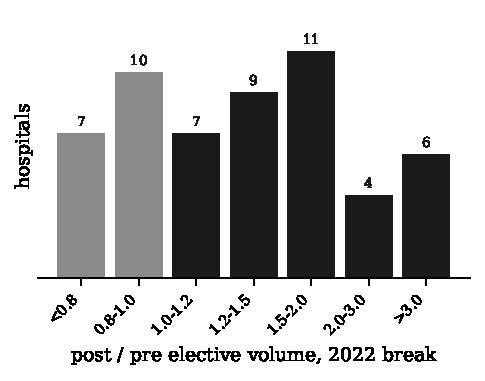
\includegraphics[width=\textwidth]{fig2_growth_histogram.pdf}
\caption{Distribution of facility-level growth ratios across the 2022 break,
reliable subset.}
\label{fig:hist}
\end{minipage}\hfill
\begin{minipage}[t]{0.5\textwidth}
\centering
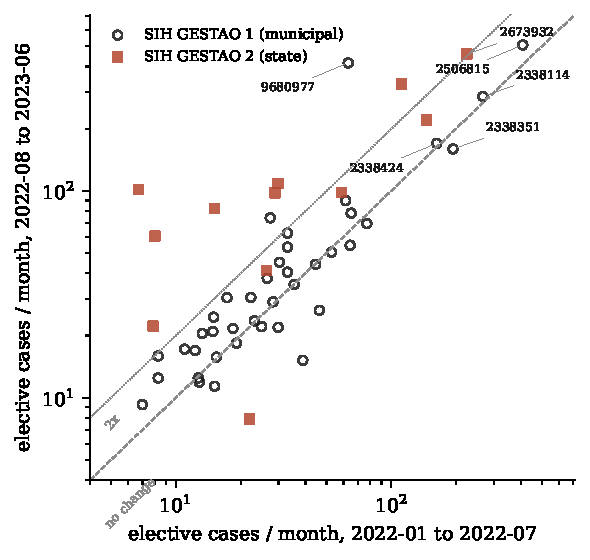
\includegraphics[width=\textwidth]{fig3_pre_post_scatter.pdf}
\caption{Monthly elective volume before and after the break, by facility, log
scale. Points on the dashed line did not change. The largest facilities lie on
or near it.}
\label{fig:scatter}
\end{minipage}
\end{figure}

Figure~\ref{fig:scatter} shows where the dispersion sits. The state's largest
elective surgical facility went from 406 to 538 cases per month, a 32 per cent
increase, and the second largest went from 321 to 263, a decline. Meanwhile a
facility performing 62 elective cases per month before the break performed 366
after it, and one performing 10 performed 95. The facilities that absorbed the
expansion were mid-sized and small units operating far below the volume of the
leaders, and after the expansion they remained below them.

This dispersion is what motivates the model. Before 2022 elective volume was concentrated in a few large facilities, and Section~\ref{sec:capbind} reports that the constructed bed-day budget was slack in aggregate. Facilities that expanded in 2022 were still operating at their new volumes in 2025, and
we do not identify what caused the expansion. The natural question is how far the realised allocation sits from a benchmark assignment.


\subsection{Falsification and robustness}

Table~\ref{tab:falsification} collects the checks that would have overturned the
result and did not.

Urgent surgical admissions move little at the break, either statewide or within
the state-administered group. Statewide urgent volume rises by 6.4 per cent
between the pre- and post-break windows and urgent volume at state-administered
facilities by 7.7 per cent, against a 38 per cent rise in the elective-to-urgent
ratio measured on admission month. Urgent volume did not fall as elective volume rose. No facility
changes its \texttt{GESTAO} code between July and August 2022, so the
concentration of the increase in state-managed units cannot be an artefact of
reclassification. Rebuilding the entire series on admission date rather than
processing month leaves the break in the same month and of the same magnitude:
the pre-window mean is 4{,}013 elective admissions per month at a ratio of
0.471 and the post-window mean is 6{,}108 at a ratio of 0.652. The submission
lag for elective admissions does not rise across the break; measured on the same
windows as the rest of the table it falls, from 0.645 months to 0.629, a change
of two and a half per cent or about half a day. The rise Section~\ref{sec:measconc} reports is between calendar 2021 and calendar 2022, which is a different
comparison and ends before the post-break window opens. Neither direction can
generate a sustained level shift of this size in any case, and the
admission-date reconstruction puts the break in the same month at the same
magnitude.

\begin{table}[t]
\centering
\caption{Falsification checks. Each row reports a quantity that would have
moved if the corresponding alternative explanation were correct.}
\label{tab:falsification}
\small
\begin{tabular}{lrrr}
\toprule
Quantity & Pre & Post & $\Delta\%$ \\
\midrule
Urgent surgical admissions, statewide & 8,554.86 & 9,102.73 & +6.4 \\
Urgent admissions, state-administered units & 3,940.86 & 4,246.09 & +7.7 \\
Hospitals with $>0$ elective cases & 105.00 & 107.36 & +2.3 \\
Concentration (HHI), elective & 479.05 & 398.19 & -16.9 \\
Elective cases, facilities absent pre-break & 0.00 & 8.00 &  \\
Facilities changing SIH management code at the break (of 101) & 0.00 & 0.00 &  \\
Mean submission lag, elective (months) & 0.65 & 0.63 & -2.6 \\
Elective/urgent ratio, by admission month & 0.47 & 0.65 & +38.4 \\
\bottomrule
\end{tabular}

\end{table}

